
\documentclass{article}

\usepackage{graphicx}
\usepackage{amsmath}
\usepackage{nccmath}
\usepackage{hyperref}

\graphicspath{ {../res/} }





%%%%%%%%%%%%%%%%%%%%%%%%%%%%%%%%%%%%%%%%%
% Lachaise Assignment
% Structure Specification File
% Version 1.0 (26/6/2018)
%
% This template originates from:
% http://www.LaTeXTemplates.com
%
% Authors:
% Marion Lachaise & François Févotte
% Vel (vel@LaTeXTemplates.com)
%
% License:
% CC BY-NC-SA 3.0 (http://creativecommons.org/licenses/by-nc-sa/3.0/)
% 
%%%%%%%%%%%%%%%%%%%%%%%%%%%%%%%%%%%%%%%%%

%----------------------------------------------------------------------------------------
%	PACKAGES AND OTHER DOCUMENT CONFIGURATIONS
%----------------------------------------------------------------------------------------

\usepackage{amsmath,amsfonts,stmaryrd,amssymb} % Math packages

\usepackage{enumerate} % Custom item numbers for enumerations

\usepackage[ruled]{algorithm2e} % Algorithms

\usepackage[framemethod=tikz]{mdframed} % Allows defining custom boxed/framed environments

\usepackage{listings} % File listings, with syntax highlighting
\lstset{
	basicstyle=\ttfamily, % Typeset listings in monospace font
}

%----------------------------------------------------------------------------------------
%	DOCUMENT MARGINS
%----------------------------------------------------------------------------------------

\usepackage{geometry} % Required for adjusting page dimensions and margins

\geometry{
	paper=a4paper, % Paper size, change to letterpaper for US letter size
	top=2.5cm, % Top margin
	bottom=3cm, % Bottom margin
	left=2.5cm, % Left margin
	right=2.5cm, % Right margin
	headheight=14pt, % Header height
	footskip=1.5cm, % Space from the bottom margin to the baseline of the footer
	headsep=1.2cm, % Space from the top margin to the baseline of the header
	%showframe, % Uncomment to show how the type block is set on the page
}

%----------------------------------------------------------------------------------------
%	FONTS
%----------------------------------------------------------------------------------------

\usepackage[utf8]{inputenc} % Required for inputting international characters
\usepackage[T1]{fontenc} % Output font encoding for international characters

\usepackage{XCharter} % Use the XCharter fonts

%----------------------------------------------------------------------------------------
%	COMMAND LINE ENVIRONMENT
%----------------------------------------------------------------------------------------

% Usage:
% \begin{commandline}
%	\begin{verbatim}
%		$ ls
%		
%		Applications	Desktop	...
%	\end{verbatim}
% \end{commandline}

\mdfdefinestyle{commandline}{
	leftmargin=10pt,
	rightmargin=10pt,
	innerleftmargin=15pt,
	middlelinecolor=black!50!white,
	middlelinewidth=2pt,
	frametitlerule=false,
	backgroundcolor=black!5!white,
	frametitle={Command Line},
	frametitlefont={\normalfont\sffamily\color{white}\hspace{-1em}},
	frametitlebackgroundcolor=black!50!white,
	nobreak,
}

% Define a custom environment for command-line snapshots
\newenvironment{commandline}{
	\medskip
	\begin{mdframed}[style=commandline]
}{
	\end{mdframed}
	\medskip
}

%----------------------------------------------------------------------------------------
%	FILE CONTENTS ENVIRONMENT
%----------------------------------------------------------------------------------------

% Usage:
% \begin{file}[optional filename, defaults to "File"]
%	File contents, for example, with a listings environment
% \end{file}

\mdfdefinestyle{file}{
	innertopmargin=1.6\baselineskip,
	innerbottommargin=0.8\baselineskip,
	topline=false, bottomline=false,
	leftline=false, rightline=false,
	leftmargin=2cm,
	rightmargin=2cm,
	singleextra={%
		\draw[fill=black!10!white](P)++(0,-1.2em)rectangle(P-|O);
		\node[anchor=north west]
		at(P-|O){\ttfamily\mdfilename};
		%
		\def\l{3em}
		\draw(O-|P)++(-\l,0)--++(\l,\l)--(P)--(P-|O)--(O)--cycle;
		\draw(O-|P)++(-\l,0)--++(0,\l)--++(\l,0);
	},
	nobreak,
}

% Define a custom environment for file contents
\newenvironment{file}[1][File]{ % Set the default filename to "File"
	\medskip
	\newcommand{\mdfilename}{#1}
	\begin{mdframed}[style=file]
}{
	\end{mdframed}
	\medskip
}

%----------------------------------------------------------------------------------------
%	NUMBERED QUESTIONS ENVIRONMENT
%----------------------------------------------------------------------------------------

% Usage:
% \begin{question}[optional title]
%	Question contents
% \end{question}

\mdfdefinestyle{question}{
	innertopmargin=1.2\baselineskip,
	innerbottommargin=0.8\baselineskip,
	roundcorner=5pt,
	nobreak,
	singleextra={%
		\draw(P-|O)node[xshift=1em,anchor=west,fill=white,draw,rounded corners=5pt]{%
		Question \theQuestion\questionTitle};
	},
}

\newcounter{Question} % Stores the current question number that gets iterated with each new question

% Define a custom environment for numbered questions
\newenvironment{question}[1][\unskip]{
	\bigskip
	\stepcounter{Question}
	\newcommand{\questionTitle}{~#1}
	\begin{mdframed}[style=question]
}{
	\end{mdframed}
	\medskip
}

%----------------------------------------------------------------------------------------
%	WARNING TEXT ENVIRONMENT
%----------------------------------------------------------------------------------------

% Usage:
% \begin{warn}[optional title, defaults to "Warning:"]
%	Contents
% \end{warn}

\mdfdefinestyle{warning}{
	topline=false, bottomline=false,
	leftline=false, rightline=false,
	nobreak,
	singleextra={%
		\draw(P-|O)++(-0.5em,0)node(tmp1){};
		\draw(P-|O)++(0.5em,0)node(tmp2){};
		\fill[black,rotate around={45:(P-|O)}](tmp1)rectangle(tmp2);
		\node at(P-|O){\color{white}\scriptsize\bf !};
		\draw[very thick](P-|O)++(0,-1em)--(O);%--(O-|P);
	}
}

% Define a custom environment for warning text
\newenvironment{warn}[1][Warning:]{ % Set the default warning to "Warning:"
	\medskip
	\begin{mdframed}[style=warning]
		\noindent{\textbf{#1}}
}{
	\end{mdframed}
}

%----------------------------------------------------------------------------------------
%	INFORMATION ENVIRONMENT
%----------------------------------------------------------------------------------------

% Usage:
% \begin{info}[optional title, defaults to "Info:"]
% 	contents
% 	\end{info}

\mdfdefinestyle{info}{%
	topline=false, bottomline=false,
	leftline=false, rightline=false,
	nobreak,
	singleextra={%
		\fill[black](P-|O)circle[radius=0.4em];
		\node at(P-|O){\color{white}\scriptsize\bf i};
		\draw[very thick](P-|O)++(0,-0.8em)--(O);%--(O-|P);
	}
}

% Define a custom environment for information
\newenvironment{info}[1][Info:]{ % Set the default title to "Info:"
	\medskip
	\begin{mdframed}[style=info]
		\noindent{\textbf{#1}}
}{
	\end{mdframed}
}
 % Include the file specifying the document structure and custom commands

%----------------------------------------------------------------------------------------
%	ASSIGNMENT INFORMATION
%----------------------------------------------------------------------------------------

\title{Cuestionario 1} % Title of the assignment

\author{David Gil Bautista\\ \texttt{DNI: 45925424M}\\ \texttt{Email: davidbautista@correo.ugr.es}} % Author name and email address

\date{Universidad de Granada --- \today} % University, school and/or department name(s) and a date

%----------------------------------------------------------------------------------------

\begin{document}

\maketitle % Print the title

%----------------------------------------------------------------------------------------
%	INTRODUCTION
%----------------------------------------------------------------------------------------

\section{Diga en una sola frase cuál cree que es el objetivo principal de la Visión por Computador. Diga también cuál es la principal propiedad de cara a los algoritmos que está presente en todas las imágenes.}
El objetivo de la Visión por Computador es que una máquina pueda llegar a analizar e interpretar una imagen.

Todos los algoritmos intentan mejorar (o cambiar) la imagen para que así sea más fácil trabajar con ella y extraer algún tipo de información.

\section{Expresar las diferencias y semejanzas entre las operaciones de correlación y convolución. Dar una interpretación de cada una de ellas que en el contexto de uso en visión por computador.}
La principal diferencia entre correlación y convolución es la propiedad asociativa, cosa que se soluciona en el caso de que la máscara de correlación sea simétrica. En este caso las operaciones presentan las siguientes propiedades:\\
 
 
\textbf{Superposition}: El resultado de la suma de los filtros es igual a la suma de los filtros individuales.

\begin{equation}
R(x + y) = R(x) + R(y)
\end{equation}

\textbf{Scaling}: El resultado de aplicar un filtro escalado es lo mismo que escalar el resultado

\begin{equation}
kR(x) = R(kx)
\end{equation}

\textbf{Shift invariance}: El resultado de aplicar un filtro cambiado equivale a cambiar el resultado de aplicar ese filtro.

\begin{equation}
R(f(x)) = f(R(x))
\end{equation}


Ambas operaciones se definen como la aplicación de un filtro, en el caso de la correlación buscamos reconocer formas o patrones y en el de la convolución la posibilidad de combinar y operar con filtros.


\section{¿Los filtros de convolución definen funciones lineales sobre las imágenes? ¿y los de mediana? Justificar la respuesta.}
Una función lineal es toda aplicación que cumple las siguientes propiedades:
Sean $V$ y $W$ espacios vectoriales sobre el mismo cuerpo  $K$. Una aplicación $T$ de $V$ en $W$ es una transformación lineal si para todo par de vectores $ u,v\in V$  y para todo escalar $k\in K$, se satisface que:
\begin{itemize}
\item $T(u+v)=T(u)+T(v)$
\item $T(ku)=kT(u)$
\end{itemize}

Para comprobar si definen o no filtros lineales comprobaremos mediante un ejemplo si cumplen las propiedades.

Para demostrar si convolución presenta una aplicación lineal probaré con  un filtro de alisamiento gaussiano.
Siendo nuestra imagen de muestra:
\begin{equation}
I=\begin{bmatrix}
1 \\ 
2 \\ 
1
\end{bmatrix}
\end{equation}
Y $u$ y $v$ nuestros filtros gaussianos:
\begin{equation}
T(u)=\begin{bmatrix}
0.15 & 0.7 & 0.15 \\ 
\end{bmatrix}
\end{equation}
\begin{equation}
T(v)=\begin{bmatrix}
0.1 & 0.8 & 0.1 \\ 
\end{bmatrix}
\end{equation}

\begin{equation}
T(u+v)=\begin{bmatrix}
0.25 & 1.5 & 0.25 \\ 
\end{bmatrix}
\end{equation} \\

Siendo $ I2 = T(u + v)$  y $I3 = T(u) + T(v)$ comprobamos que sean iguales:
\begin{equation}
I2 = \begin{bmatrix}
1 \\ 
2 \\ 
1
\end{bmatrix}*\begin{bmatrix}
0.25 & 1.5 & 0.25 \\ 
\end{bmatrix}=3.5
\end{equation}
\begin{equation}
I3 = \begin{bmatrix}
1 \\ 
2 \\ 
1
\end{bmatrix}*\begin{bmatrix}
0.15 & 0.7 & 0.15 \\ 
\end{bmatrix}+\begin{bmatrix}
1 \\ 
2 \\ 
1
\end{bmatrix}*\begin{bmatrix}
0.1 & 0.8 & 0.1 \\ 
\end{bmatrix}= 1.7 + 1.8 = 3.5
\end{equation}

Comprobando $T(kv) = kT(v)$:
\begin{equation}
T(2v) = \begin{bmatrix}
0.2 & 1.6 & 0.2 \\ 
\end{bmatrix}*\begin{bmatrix}
1 \\ 
2 \\ 
1
\end{bmatrix}=3.6 = 2* T(v)
\end{equation}

Para el caso del filtro mediano probaremos con una matriz más grande para que sea más fácil de comprobar. Usando las siguientes matrices:

\begin{equation}
I = \begin{bmatrix}
1 & 1 & 2 & 15 & 34 \\ 
\end{bmatrix}
\end{equation}

\begin{equation}
J = \begin{bmatrix}
6 & 7 & 7 & 8 & 9 \\ 
\end{bmatrix}
\end{equation}

\begin{equation}
(I+J) = \begin{bmatrix}
7 & 8 & 9 & 23 & 43 \\ 
\end{bmatrix}
\end{equation}

Siendo $m(X)$ la mediana de una matriz $X$ tenemos que:
\begin{equation}
m(I) = 2 ,\\\ m(J) = 9
\end{equation}

\begin{equation}
m(I)+m(J) = 11
\end{equation}

\begin{equation}
m(I + J) = 9
\end{equation}

Sabiendo que un filtro de mediana no cumple la primera propiedad ya podemos determinar que no define una función lineal sobre una imagen.

\section{Una operación de máscara que tipo de información usa, ¿local o global? Justificar la respuesta}
Local. Cada vez que aplicamos la máscara estamos trabajando sobre una zona concreta de la imagen con unos píxeles determinados, tan sólo operamos con la información esos píxeles y al cambiar de zona trabajamos con otros distintos cuya información puede ser distinta.

\section{¿De qué depende que una máscara de convolución pueda ser implementada de forma separable por filas y columnas? Justificar la respuesta}

Deben existir dos matrices de una dimensión $v, w$ cumpliendo que $IMG * f * v = IMG(f * v)$ siendo $(f*v)$ la matriz que representa ese producto matricial.


\section{Para implementar una función que calcule la imagen gradiente de una imagen cabe plantearse dos alternativas:}

\subsection{Primero alisar la imagen y después calcular las derivadas sobre la imagen alisada }

\subsection{Primero calcular las imágenes derivadas y después alisar dichas imágenes. }


\textbf{Discutir y decir cuál de las estrategias es la más adecuada, si alguna lo
es, tanto en el plano teórico como en el de la implementación. Justificar
la decisión.}\\

Una imagen gradiente nos permite encontrar los saltos bruscos que hay en la imagen y de esta forma encontrar los bordes. En caso de tener una imagen con ruido, al hacer el gradiente vamos a resaltar el ruido y al alisar tan solo vamos a difuminar las manchas. En el caso de alisar primero quitamos todo el ruido haciendo una media de los valores que debería haber en esos puntos y al hacer el gradiente a esta imagen los errores que puedan llegar a percibirse van a ser menos intensos.
\\
Para probar si esto es cierto o no lo comprobaremos con el siguiente ejemplo:

\begin{figure}[h]
\vspace{0.5cm}
\centering
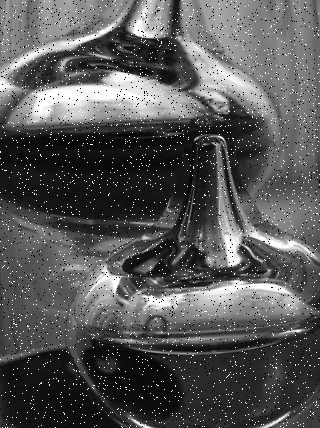
\includegraphics[scale=0.45]{noise.png}
\caption{Original image}	
\end{figure}

\begin{figure}[h]
\begin{minipage}[b]{0.5\linewidth}
\centering
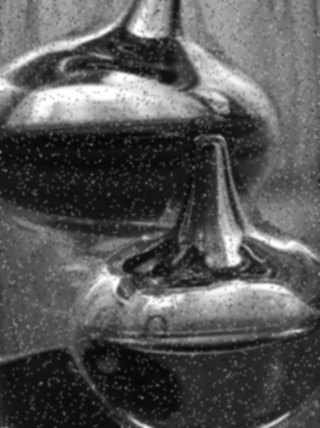
\includegraphics[scale=0.45]{firstblur.PNG}
\caption{First smooth}	
\end{minipage}
\begin{minipage}[b]{0.5\linewidth}
\centering
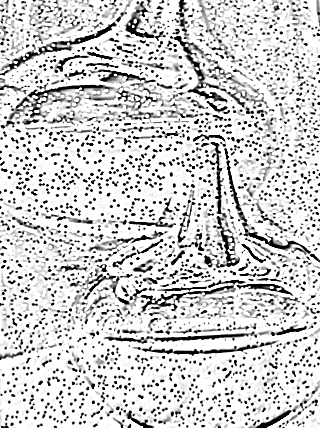
\includegraphics[scale=0.45]{thensobel.PNG}
\caption{then get sobels}
\end{minipage}
\end{figure}

\begin{figure}[h]
\begin{minipage}[b]{0.5\linewidth}
\centering
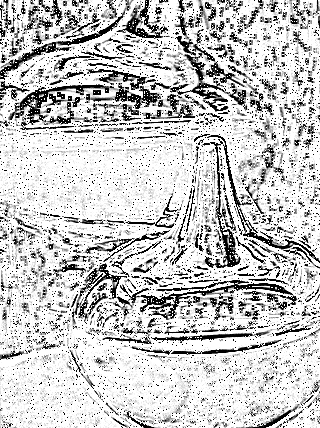
\includegraphics[scale=0.45]{firstsobel.PNG}
\caption{First get sobels}	
\end{minipage}
\begin{minipage}[b]{0.5\linewidth}
\centering
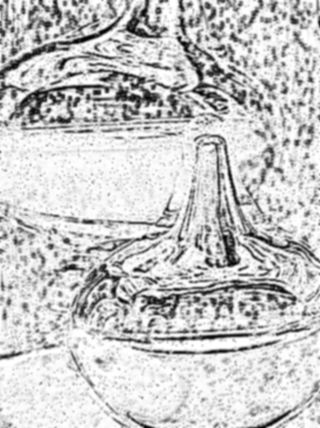
\includegraphics[scale=0.45]{thenblur.PNG}
\caption{then smooth}
\end{minipage}
\end{figure}

\newpage
Para un filtro de desenfoque gaussiano con tamaño de kernel de 5x5 y un filtro de detección de bordes laplaciano con un tamaño de kernel de 5x5 hemos obtenido los resultados anteriores.

Aplicando la teoría, al alisar primero estamos quitando las imperfecciones, por lo que al detectar los bordes no deberíamos encontrar ruido. La realidad es que si la imagen es pequeña, al alisar estamos haciendo que el ruido ocupe más espacio, por lo que será más reconocible al detectar los bordes. En caso de hacerlo a la inversa, el ruido estará en pixeles determinados que estarán rodeados de un color plano el cual hará que al hacer la media ese pixel tome el valor de los contiguos y por tanto se eliminará casi al completo el ruido.

\newpage
\section{Verificar matemáticamente que las primeras derivadas (respecto de x e y) de la Gaussiana 2D se puede expresar como núcleos de convolución separables por filas y columnas. Interpretar el papel de dichos núcleos en el proceso de convolución.}

Para demostrar esto tomaremos la expresión de una operación gaussiana y la descompondremos para probar que es separable.


\begin{align*}
& G_{\sigma}(x,y) = \frac{1}{2\pi\sigma^2} e^{-\frac{x^2+y^2}{2\sigma^2}}\\
\\
& G_{\sigma}(x,y) = \frac{1}{2\pi\sigma^2}e^{\frac{-x^2}{2\sigma^2}+{\frac{-y^2}{2\sigma^2}}}\\
\\
& G_{\sigma}(x,y) = \frac{1}{2\pi\sigma^2}e^{\frac{-x^2}{2\sigma^2}}e^{\frac{-y^2}{2\sigma^2}}\\
\\
& G_{\sigma}(x,y) = \sqrt{\frac{1}{2\pi\sigma^2}}^2e^{\frac{-x^2}{2\sigma^2}}e^{\frac{-y^2}{2\sigma^2}}\\
\\
& G_{\sigma}(x,y) = \sqrt{\frac{1}{2\pi\sigma^2}}\sqrt{\frac{1}{2\pi\sigma^2}}e^{\frac{-x^2}{2\sigma^2}}e^{\frac{-y^2}{2\sigma^2}}\\
\\
& G_{\sigma}(x,y) = \frac{1}{\sqrt{2\pi}\sigma}\frac{1}{\sqrt{2\pi}\sigma}e^{\frac{-x^2}{2\sigma^2}}e^{\frac{-y^2}{2\sigma^2}}\\
\\
& G_{\sigma}(x,y) =\Bigg( \frac{1}{\sqrt{2\pi}\sigma}e^{\frac{-x^2}{2\sigma^2}}\Bigg) \Bigg(\frac{1}{\sqrt{2\pi}\sigma}e^{\frac{-y^2}{2\sigma^2}}\Bigg)\\
\\
& G_{\sigma}(x,y) = G_{\sigma}(x)G_{\sigma}(y)
\end{align*}

De esta forma podemos ver que podemos tratar la Gaussiana 2D como producto de la convolución de filas y columnas.

Haciendo las derivadas parciales de $G_{}\sigma (x,y)$ tenemos que:

\begin{equation}
\frac{\partial}{\partial x} G_{\sigma}(x,y) = -\frac{ e^{-x^2/(2 \sigma^2) - y^2/(2 \sigma^2)} x}{2\pi\sigma^4}
\end{equation}

\begin{equation}
\frac{\partial}{\partial y} G_{\sigma}(x,y) = -\frac{ e^{-x^2/(2 \sigma^2) - y^2/(2 \sigma^2)} y}{2\pi\sigma^4}
\end{equation}

Haciendo la primera derivada de $G_{\sigma}(x)$ y de $G_{\sigma}(y)$ obtenemos lo siguiente:

\begin{equation}
\frac{\partial}{\partial x} G_{\sigma}(x) = -\frac{e^{-\frac{x^2}{(2 \sigma^2)}}x}{\sqrt{2 \pi}\sigma^3}
\end{equation}
\begin{equation}
\frac{\partial}{\partial y} G_{\sigma}(y) = -\frac{e^{-\frac{y^2}{(2 \sigma^2)}}y}{\sqrt{2 \pi}\sigma^3}
\end{equation}

\newpage

Al calcular las derivadas parciales podemos ver que la función que obtenemos es la misma para la derivada de $x$ e $y$, pero cambia el término que multiplica a la exponencial en el numerador. Del mismo modo obtenemos lo mismo al derivar el filtro Gaussiano en función de $x$ e $y$, en este caso cambiamos la $x$ o la $y$ en toda la función. Al representar las derivadas obtenemos la misma función con un eje cambiado.


\begin{figure}[h]
\vspace{0.5cm}
\centering
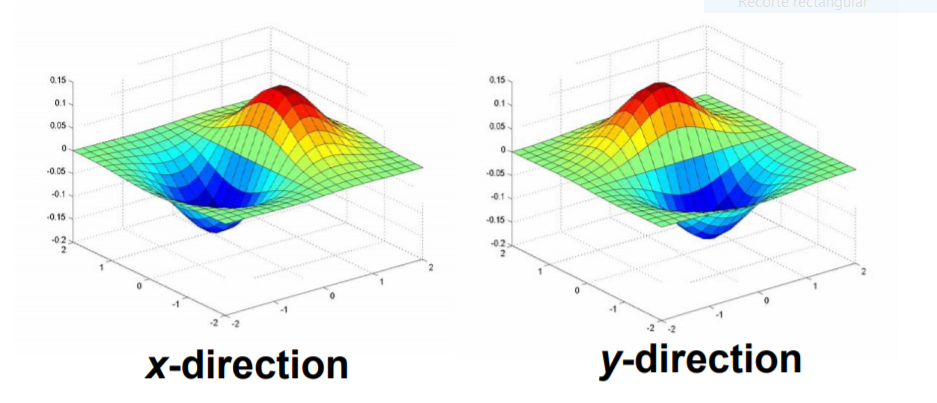
\includegraphics[scale=0.7]{partial.png}
\caption{Gaussian derivatives}	
\end{figure}


\section{Verificar matemáticamente que la Laplaciana de la Gaussiana se puede implementar a partir de núcleos de convolución separables por filas y columnas. Interpretar el papel de dichos núcleos en el proceso de convolución. }

La función Laplaciana de la Gaussiana se define como la suma de las segundas derivadas de la función Gaussiana. En el apartado anterior calculamos las derivadas parciales en $x$ e $y$, por lo que volveremos a derivar estas y comprobarlas con la función Laplaciana para comprobar si son equivalentes.
Siendo la función Laplaciana:
\begin{equation}
\nabla^2 G_{\sigma}(x,y) = \frac{\partial^2 G_{\sigma}(x,y)}{\partial x^2} + \frac{\partial^2 G_{\sigma}(x,y)}{\partial y^2}
\end{equation}


Y las segundas derivadas parciales de la función Gaussiana:
\begin{equation}
\frac{\partial^2}{\partial x^2} G_{\sigma}(x,y) = \frac{(x^2-\sigma^2)e^{-\frac{x^2+y^2}{2\sigma^2}}}{2\pi\sigma^6}
\end{equation}

\begin{equation}
\frac{\partial^2}{\partial y^2} G_{\sigma}(x,y) = \frac{(y^2-\sigma^2)e^{-\frac{x^2+y^2}{2\sigma^2}}}{2\pi\sigma^6}
\end{equation}

Desarrollando podemos obtener lo siguiente:

\begin{align*}
& \nabla^2 G_{\sigma}(x,y) = \frac{(x^2-\sigma^2)e^{-\frac{x^2+y^2}{2\sigma^2}}}{2\pi\sigma^6} + \frac{(y^2-\sigma^2)e^{-\frac{x^2+y^2}{2\sigma^2}}}{2\pi\sigma^6}\\
\\
& \nabla^2 G_{\sigma}(x,y) = \Bigg( \frac{(x^2-\sigma^2)e^{-\frac{x^2}{2\sigma^2}}}{2\pi\sigma^6}e^{-\frac{y^2}{2\sigma^2}}\Bigg) + \Bigg( \frac{(y^2-\sigma^2)e^{-\frac{y^2}{2\sigma^2}}}{2\pi\sigma^6}e^{-\frac{x^2}{2\sigma^2}}\Bigg)\\
\end{align*}

Al igual que en el ejercicio anterior cada derivada representa la función en un eje por lo que la suma de las dos nos proporciona la función Laplaciana, la cuál tiene la siguiente forma:

\begin{figure}[h]
\vspace{0.5cm}
\centering
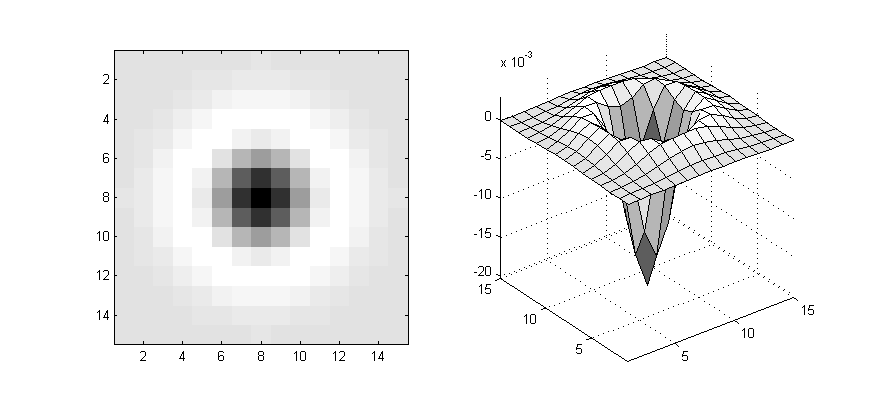
\includegraphics[scale=0.6]{laplac.png}
\caption{Laplacian function representation}	
\end{figure}



\section{¿Cuáles son las operaciones básicas en la reducción del tamaño de una imagen? Justificar el papel de cada una de ellas. }
En caso de querer reducir el tamaño de una imagen buscamos la forma de representar en una matriz más pequeña la misma información que teníamos en otra más grande. La forma más sencilla de hacer esto es interpolando píxeles de la imagen original y llevándolos a otra más pequeña o escalando la imagen con una transformación afín en la que la matriz de convolución tenga valores comprendidos entre 0 y 1 en la diagonal principal. De esta forma los píxeles tienen una nueva posición en la imagen, pero puede pasar que en una posición en la que tuviéramos solo un valor ahora tengamos cuatro, por lo que también se debe decidir lo que se hará cuando se tenga una superposición de píxeles.

Existen algoritmos inteligentes que nos permiten escalar imágenes preservando el valor original que encontramos en ciertas zonas de interés para no perder información relevante cuando escalemos una imagen.

URL escalado de imágenes inteligente: \href{http://nparashuram.com/seamcarving/}{Seam Carving}

\section{- ¿Qué información de la imagen original se conserva cuando vamos subiendo niveles en una pirámide Gaussiana? Justificar la respuesta. }

Las bajas frecuencias,ya que al ir subiendo niveles en la pirámide gaussiana reescalamos la imagen de forma que en cada nivel tenemos menos información que en el anterior, y esto es lo mismo que eliminar las frecuencias altas.

\section{¿Qué información podemos extraer de la pirámide Gaussiana y la pirámide Laplaciana de una imagen? ¿Qué nos aporta cada una de ellas? Justificar la respuesta. }
La ambas pirámides nos aportan una imagen más pequeña que la original, la diferencia es que en el caso de la Laplaciana al reescalarla al tamaño original podemos recuperar las altas frecuencias que se pierden al reescalar la imagen. En el caso de la Gaussiana obtenemos tan solo las bajas frecuencias ya que no guardamos ninguna información y al reescalar al tamaño original tan sólo interpolamos los píxeles de la imagen pequeña.

\section{¿Podemos garantizar una perfecta reconstrucción de una imagen a partir de su pirámide Laplaciana? Dar argumentos y discutir las opciones que considere necesario.}
No, para ello tomaremos el ejemplo de una imagen con una recta diagonal. Cuando la imagen es muy grande podemos combatir el \textit{aliasing} usando los píxeles cercanos para difuminar el salto tan brusco. Al subir niveles en la pirámide Laplaciana guardaremos las altas frecuencias, es decir, los bordes de la imagen que en este ejemplo sería equivalente a guardar el \textit{aliasing}. Una vez tenemos la imagen pequeña con toda la información de las altas frecuencias, al reescalarla recuperaremos la diagonal que teníamos pero no con el \textit{antialiasing} que podríamos haber aplicado previamente, pues al reducir la imagen las bajas frecuencias del \textit{antialiasing} se mezclan con los otros píxeles y al reescalar al tamaño original no hay forma de recuperarlas.

\begin{figure}[h]
\begin{minipage}[b]{0.3\linewidth}
\centering
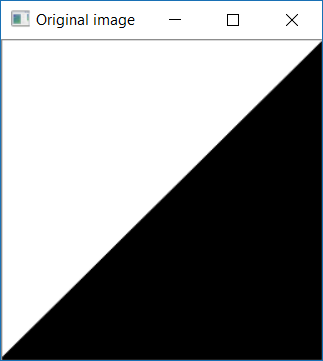
\includegraphics[scale=0.4]{img1.PNG}
\caption{Img original}	
\end{minipage}
\begin{minipage}[b]{0.3\linewidth}
\centering
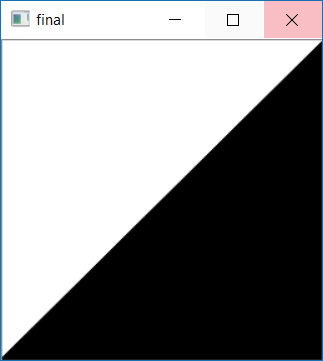
\includegraphics[scale=0.4]{img2.PNG}
\caption{Laplacian recons}
\end{minipage}
\begin{minipage}[b]{0.3\linewidth}
\centering
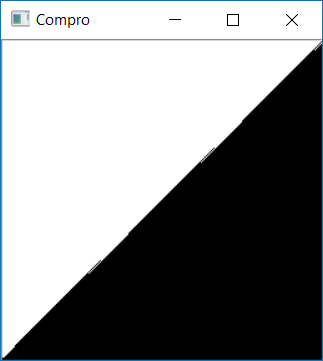
\includegraphics[scale=0.4]{img3.PNG}
\caption{Compare}
\end{minipage}
\end{figure}

Al subir en la pirámide laplaciana podemos ver que obtenemos una imagen muy similar a la original y que a priori no se han perdido datos. Cuando comparamos las dos imágenes podemos ver que presenta dientes de sierra en la diagonal, y que por tanto la reconstrucción con la pirámide laplaciana no nos ha devuelto la imagen original.

\section{En OpenCV solo se pueden calcular máscaras Sobel de hasta dimensión 7x7 ¿Por qué? De una explicación razonable a este hecho y diga cómo influye en el cálculo con máscaras de mayor tamaño. Justificar la respuesta}
Siendo $k = 2\sigma + 1$ con $k$ representando el tamaño del kernel tenemos que $k = 7$ en caso de que $\sigma = 3$, $\sigma$ representa la varianza en una muestra, en caso de tener una varianza alta los datos están más alejados de la media y dispersos. Sabiendo que con un $\sigma = 3$ y representándolo en una campana de Gauss obtenemos el 96\% de la muestra, determinamos que el tamaño óptimo para calcular una máscara Sobel es $k = 7$ . Aumentar el tamaño de la máscara tendría cambios insignificantes. 

\section{Cuales son las contribuciones más relevantes del algoritmo de Canny al cálculo de los contornos sobre una imagen?. ¿Existe alguna conexión entre las máscaras de Sobel y el algoritmo de Canny? Justificar la respuesta}
El algoritmo para detección de bordes de Canny se basa en el cálculo del gradiente en los píxeles pero además añade lo siguiente:
\begin{itemize}
\item \textbf{Non-maximum suppression}: Comprueba los puntos de los bordes y en caso de tener varios (borde ancho), elimina todos menos el máximo para conseguir un borde más fino.
\item \textbf{Linking and thresholding (hysteresis)}: Una vez se hayan los bordes define dos umbrales, uno mayor y otro menor. Una vez tenemos este umbral volvemos a analizar la imagen, en caso de que un pixel se encuentre en el umbral superior quiere decir que dicho píxel forma parte de un borde, en caso de que pertenezca al umbral inferior no será un borde.Lo que hace que este detector sea tan importante es lo que pasa cuando un pixel se encuentra entre ambos umbrales, en este caso, Canny dice que dicho pixel pertenece a la unión entre dos límites en la dirección del gradiente. Sabiendo ambos límites podemos usar ese pixel para unir dos bordes.
\end{itemize}

Una máscara Sobel es aplica un gradiente a cada pixel, al aplicar una máscara de este tipo podemos reconocer los bordes horizontales y verticales. El algoritmo de Canny implementa una máscara de gradiente para detectar los bordes y la combina con las operaciones de las que he hablado anteriormente.


\section{Suponga que le piden implementar un algoritmo para el cálculo de la derivada de primer y segundo orden sobre una imagen usando un filtro gaussiano cualesquiera. Enumere y explique los pasos necesarios para llevarlo a cabo.}
Usando convolución se podrían calcular las derivadas del filtro gaussiano y aplicarlo directamente a la imagen sin necesidad de alisar primero y luego derivar.


\section{Algunas referencias}
\begin{itemize}
\item\href{http://cmuems.com/excap/readings/forsyth-ponce-computer-vision-a-modern-approach.pdf}{Computer vision a modern approach}

\item\href{https://towardsdatascience.com/a-basic-introduction-to-separable-convolutions-b99ec3102728}{Separable convolutions}


\item Herramientas usadas para ejercicio 6:\\
\href{https://pinetools.com/image-edge-detection}{Edge detection}

\href{https://pinetools.com/blur-image}{Blur images}

\item \href{https://ece.uwaterloo.ca/~nnikvand/Coderep/Codes%20for%20QoMeX%202011%20paper/iwssimcode/matlabPyrTools/TUTORIALS/pyramids.html#9}{Pyramids}


\end{itemize}







\end{document}
